\documentclass[9pt]{beamer}
\usepackage[english, frenchb]{babel}
\usepackage{pgf}
\usepackage{amsmath}
\usepackage{amsthm}
\usepackage{amsfonts}
\usepackage{dsfont}
\usepackage[latin1]{inputenc}
\usepackage[T1]{fontenc}
\usepackage{graphics,color,bbm}
\usepackage{array}
\usepackage{subfigure}
\usepackage[english,frenchb]{babel}
\usepackage{beamerthemesplit}
\usepackage[latin1]{inputenc}
\usepackage[T1]{fontenc}
\usepackage{amsmath}
\usepackage{amsfonts}
\usepackage{subfigure}
\usepackage{amsthm}
\usepackage{amssymb}
\usepackage{media9}
\usepackage{multimedia}
\usepackage{comment}
\usepackage{epstopdf}
\usepackage{mathrsfs}
\usepackage{color}
\usepackage{listings}
\usepackage{comment}
\usepackage{animate}

\theoremstyle{plain} \newtheorem{Theo}{Theorem}[section]
\theoremstyle{plain} \newtheorem{Prop}{Proposition}[section]
\theoremstyle{plain} \newtheorem{Def}{Definition}[section]
\theoremstyle{plain} \newtheorem{Lem}{Lemma}[section]
\title{\textcolor{red}{The perceptron}}
\author{\textcolor{red}{\underline{TEAM POTATO CLOCK}\\ \vspace{0.1cm} Erin Edkins\\Alex Ludert\\Gautier PICOT\\}}
%\institute{\textcolor{red}{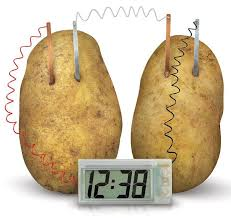
\includegraphics[width=2cm]{pot.jpg}\\ Department of Mathematics, University of Hawai'i at Manoa}}
\date{ \\
\textcolor{red}{ICS 635\\University of Hawai'i\\ September 2, 2016}}
\addtobeamertemplate{footline}{\insertframenumber/\inserttotalframenumber}

\titlegraphic{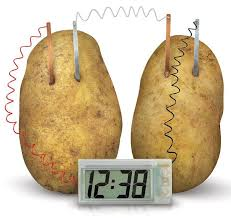
\includegraphics[width=2.5cm]{pot.jpg}}

\begin{document}
{
%\usebackgroundtemplate{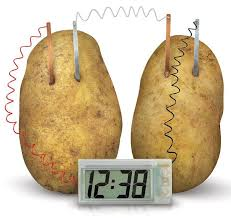
\includegraphics[height=\paperheight]{pot.jpg}}
\frame{\titlepage}
}	

\frame
{
\frametitle{\textcolor{red}{The Perceptron Algorithm}}
Our Perceptron program classifies of a set of $N$  \textit{\textcolor{red}{two-dimensional}} points $(x_j, y_j)$ with label $l_j=\pm 1$ by using a \textit{\textcolor{red}{learning rate}} $<c\leq 1$ (0.5 by default).

\begin{itemize}
\item<2-9>\textit{\textcolor{red}{Datas}}: $(x_j, y_j, l_j), \ 1\leq j \leq N $
\item<3-9>\textit{\textcolor{red}{Points}}: $P_j=(1,x_j, y_j), \ 1\leq j \leq N $
\item<4-9> Initialize the \textit{\textcolor{red}{weight}} vector $w=(0,0,0)$
\item<5-9> Initialize the \textit{\textcolor{red}{outputs}} $y_j=1,  \ 1\leq j \leq N $
\item<6-9>
\begin{tabular}{>{\centering\arraybackslash}m{.35\textwidth} >{\centering\arraybackslash}m{.3\textwidth}}
    Transfer $\theta$: \textit{\textcolor{red}{Step function}}  & 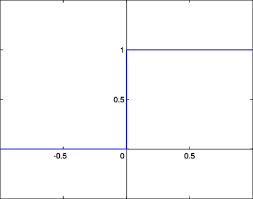
\includegraphics[width=2cm]{step.png}\\
\end{tabular}
\item<7-9> While the classification is not achieved
\begin{itemize}
\item Initialize \texttt{wrong}$=0$
\item For each  point $P_j$, calculate the \textit{\textcolor{red}{new label}} $y_j=\theta(w\cdot P_j )$
		\item If $y_j \neq l_j$, \textit{\textcolor{red}{update the weight}} $w+= c*y_j*P_J$ and \texttt{wrong}$+=1$
\end{itemize}
\item <8-9> Classification is \textit{\textcolor{red}{achieved}} if \texttt{wrong}$=0$
\item []<9-9> \underline{Remark}: to guarantee that the algorithm stops, we  \textit{\textcolor{red}{limit the while loop loops}} (at most 50 iterations by default).
\end{itemize}
}
\frame
{
\frametitle{\textcolor{red}{The Data Faker Generator }}
To test our algorithm, we have implemented a \textit{\textcolor{red}{Data Fake Generator.}}
\begin{itemize}
\item<2-5> Generates a cloud of random 2D points separated by a line 
\begin{itemize}
\item <3-5> Random \textit{\textcolor{red}{slope}} $ -1 \leq m \leq 1$ and  random y-intercept $ -1 \leq b \leq 1$  by default.
\item <4-5> The user may enter desired values for $m$ and $b$.
\end{itemize}
\item[]<5-5>
\begin{figure}
\centering
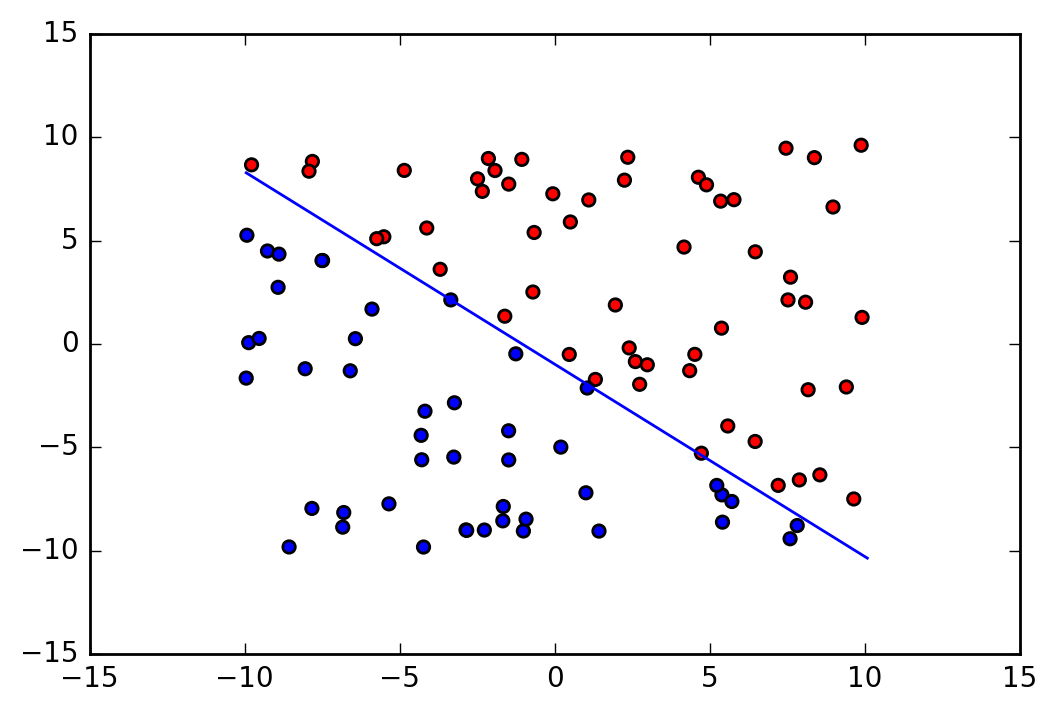
\includegraphics[width=5cm]{data_faker_p_N100.png}
\caption{A collection 100 points linearly separated}
\end{figure}
\end{itemize}
}

\frame
{
\frametitle{Convergence of the algorithm: the linearly separable case}
The algorithm \textit{\textcolor{red}{converges}} when the classified datas can be separated by a line.
\centering
\animategraphics[loop,controls,width=5cm]{2}{perceptron_animation-}{0}{17}

\vspace{0.2cm}

In this animation, the \textit{\textcolor{green}{green line}} shows the line defined by the weight vector $w$. Through the execution of the algorithm, the line \textit{\textcolor{red}{stabilizes}} $\iff$ the weight vector is \textit{\textcolor{red}{no longer}} updated $\iff$ the algorithm \textit{\textcolor{red}{converges}}. 
}

\frame
{
\frametitle{Divergence of the algorithm: the non linearly separable case}
The algorithm \textit{\textcolor{red}{diverges}} when the classified datas can not be separated by a line.
\centering
\animategraphics[loop,controls,width=5cm]{2}{xor-}{0}{10}

\vspace{0.2cm}

In this animation, the \textit{\textcolor{green}{green line}} shows the line defined by the weight vector $w$. Through the execution of the algorithm, the line \textit{\textcolor{red}{does not stabilize}} $\iff$ the weight vector \textit{\textcolor{red}{keeps being  updated}} $\iff$ the algorithm \textit{\textcolor{red}{diverges}}. 
}

\frame
{
\frametitle{Thank you...}
...Mister Rosenblatt!
\vspace{0.2cm}
\begin{figure}
\centering
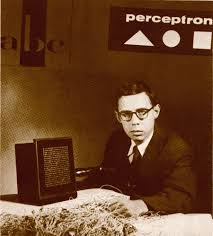
\includegraphics[width=5cm]{Rosen.jpg}
\end{figure}
}



\end{document}














\begin{comment}
\begin{itemize}
\item<2-8> Control theory is a branch of mathematics that studies the properties of \textit{\textcolor{red}{control systems}} i.e \textit{\textcolor{red}{dynamical systems whose behavior can be modified by a command}}\\
\item<3-8>General Mathematical formalism of a control system:
 \[ \dot x(t) =f(t,x(t),u(t))\] where
\begin{itemize}
\item <4-8> $t \in [t_0 t_f]$ is the \textcolor{red}{time} variable,
\item <5-8> $x$ is the \textcolor{red}{state} variable defined on $[t_0 t_f]$ and valued in a smooth variable $M$,
\item <6-8> $u$ is a measurable bounded function defined on $[t_0 t_f]$, valued in a smooth variable $U$, called the \textcolor{red}{control} variable,
\item <7-8> $f:\mathbf{R}\times M \times U \rightarrow TM$  is a \textcolor{red}{smooth} application.
\end{itemize}
\item <8-8>Goal: Bring the state variable from a given \textcolor{red}{initial} condition to a given \textcolor{red}{final} condition 
i.e solve a \textcolor{red}{boundary value} problem
\[
\left \lbrace  \begin{array}{c}  \dot x(t)=f(t,x(t),u(t))\\ 
  x(t_0)=x_{0} \in M, \ x(t_f)=x_f \in M. \end{array} \right.
\]
\end{itemize}
\end{comment}













